\documentclass[style=upen, size=14pt]{powerdot}
\usepackage{natbib}
\usepackage{bibentry}
\usepackage{mathtools}
\definecolor{arany}{RGB}{255,242,0}
\hypersetup{backref=page}
\hypersetup{
    colorlinks=true,
    linkcolor=cyan,
    citecolor=cyan,
    filecolor=magenta,      
    urlcolor=cyan}
% \pdsetup{trans=Split}
\usepackage{graphicx}
\usepackage{amsmath}
\DeclareMathOperator*{\argmax}{argmax}
\DeclareMathOperator*{\argmin}{argmin}
\DeclareMathOperator*{\softmax}{softmax}
\DeclareMathOperator{\sign}{sign}
\usepackage{amssymb}
\usepackage{stmaryrd}
\usepackage[latin2]{inputenc}
%\usepackage[magyar]{babel}
%\usepackage{euler}
\usepackage{tikz}
\usetikzlibrary{matrix}
\usepackage{tikz-qtree}
\usepackage{tikz-dependency}
\usepackage{linguex}
\usepackage{amsthm}
\usepackage{amsmath}
%\tikzset{every tree node/.style={align=center,anchor=north}}
%\usepackage{tabularx}
%\usepackage{threeparttable}
%\usepackage{color}
%\selectlanguage{english}
%\frenchspacing
\usepackage{algpseudocode}
\usepackage{algorithm}
\newcommand\varlist{,\makebox[1em][c]{.\hfil.\hfil.},}
\newcommand{\nd}{\noindent}
\newcommand{\Val}{\mathop{\mathit{Val}}}
\newcommand{\gold}{\color{arany}}
%\usepackage{tikz}
%\usepackage{tikz-qtree}
%\newcommand{\qed}{\hfill\mbox{\raggedright \rule{.1in}{.1in}}}
\def\es{\mathbin\land}
\theoremstyle{definition}
\newtheorem*{definition}{Definition}
\newtheorem{axioma}{Axiom}
\newtheorem{tetel}{Theorem}
\newtheorem{prop}{Proposition}
\newtheorem{lemma}{Lemma}
\begin{document}

\title{Natural Language Processing\\~~\\Lecture 11\\Contextual embeddings and
  transformers}
% \author{}

\date{2021}
\maketitle

\begin{slide}[toc=Embedding limitations]{Word embedding limitations}
  Traditional co-occurrence matrix-based word vectors and the first generation
  of neural word embeddings had several important limitations:
  \begin{itemize}
  \item \emph{\gold Context independence:} One surface form has only one
    representation. E.g., \emph{bank} will have the same embedding in the
    sentences\medskip

    \emph{I went to my bank to withdraw some money.}\medskip


    \emph{We explored the river bank.}\medskip

    even though the two meanings are clearly different.
  \end{itemize}
\end{slide}

\begin{slide}[toc=]{Word embedding limitations cont.}
  \begin{itemize}
  \item \emph{\gold Words are black boxes:} Words have internal structure: they
    consist of characters and can be composed of several morphemes, but
    Word2vec, GloVe etc. ignore word internals.
  \item \emph{\gold No useful representation for unseen or rare words:} As words
    are treated as black boxes, these models cannot produce useful
    representations for words that do not occur or are very rare in the training
    corpus.
  \item \emph{\gold Good coverage requires huge model dimensions:} A word gets a
    meaningful representation only if it's explicitly included in the vocabulary
    of the model, but the memory consumption is typically a linear function of
    the covered vocabulary.
  \end{itemize}
\end{slide}

\begin{slide}[toc=]{Word embedding limitations cont.}
  The problem of utilizing internal word structure, handling OOV words and
  reducing the vocabulary size was efficiently solved both by
  \begin{itemize}
  \item fastText embeddings, and, especially,
  \item subword embeddings,
  \end{itemize}
  but these embeddings were still \emph{\gold static}, i.e., mapped tokens
  of the same form to the same embedding vector.

  One of the most important recent developments in NLP has been the appearance
  of \emph{\gold contextual embeddings}, which, in contrast, can vary the
  embedding of the same surface form from context to context to reflect
  linguistic differences.
\end{slide}

\begin{slide}[toc=Contextual embeddings]{Contextual embeddings}
  \emph{\gold Contextual embeddings} are word or subword representations
  produced by deep networks (commonly LSTM or self-attention based) that are
  (pre)trained on self-supervised, broadly language modeling objectives.
  \bigskip

  Unlike static embeddings, these representations cannot be simply stored and
  deployed in the form of lookup tables, because they are \emph{dynamically}
  computed for each token based on their context: For a
  $\mathbf{w} = \langle w_1,\dots ,w_n \rangle$ input token sequence the network
  produces an
  $$
  E(\langle w_1,\dots ,w_n \rangle) = \langle
  E_\mathbf{w}(w_1),\dots,E_\mathbf{w}(w_n)\rangle
  $$
  embedding sequence.
\end{slide}

\begin{slide}[toc=]{Contextual embeddings cont.}
  Because of this dynamic nature, the network itself has to be used as a
  \emph{\gold feature extractor module}.\bigskip

  The envisaged use of contextual embedding producing networks in NLP is similar
  to the role of processing pipelines in traditional NLP: they are supposed to
  produce feature vectors that are useful for downstream tasks, in fact, the
  hope is that only little further processing (e.g., in the form of shallow
  neural networks) is needed to build useful NLP models.
\end{slide}

\begin{slide}[toc=ELMo]{ELMo (Embeddings from Language Models)}
  ELMo \citep{peters2018deep}, the historically first important contextual
  embedding model, learns word representations via standard one-directional
  language modeling tasks.\bigskip

  The architecture starts with producing context-independent embeddings using
  character-level convolutions, and then uses forward and backward bidirectional
  LSTM layers (their number, $n$, is a changeable hyperparameter) to predict the
  next/previous token via weight-shared softmax layers:
\end{slide}

\begin{slide}[toc=]{ELMo cont.}
  \hspace{0.3cm}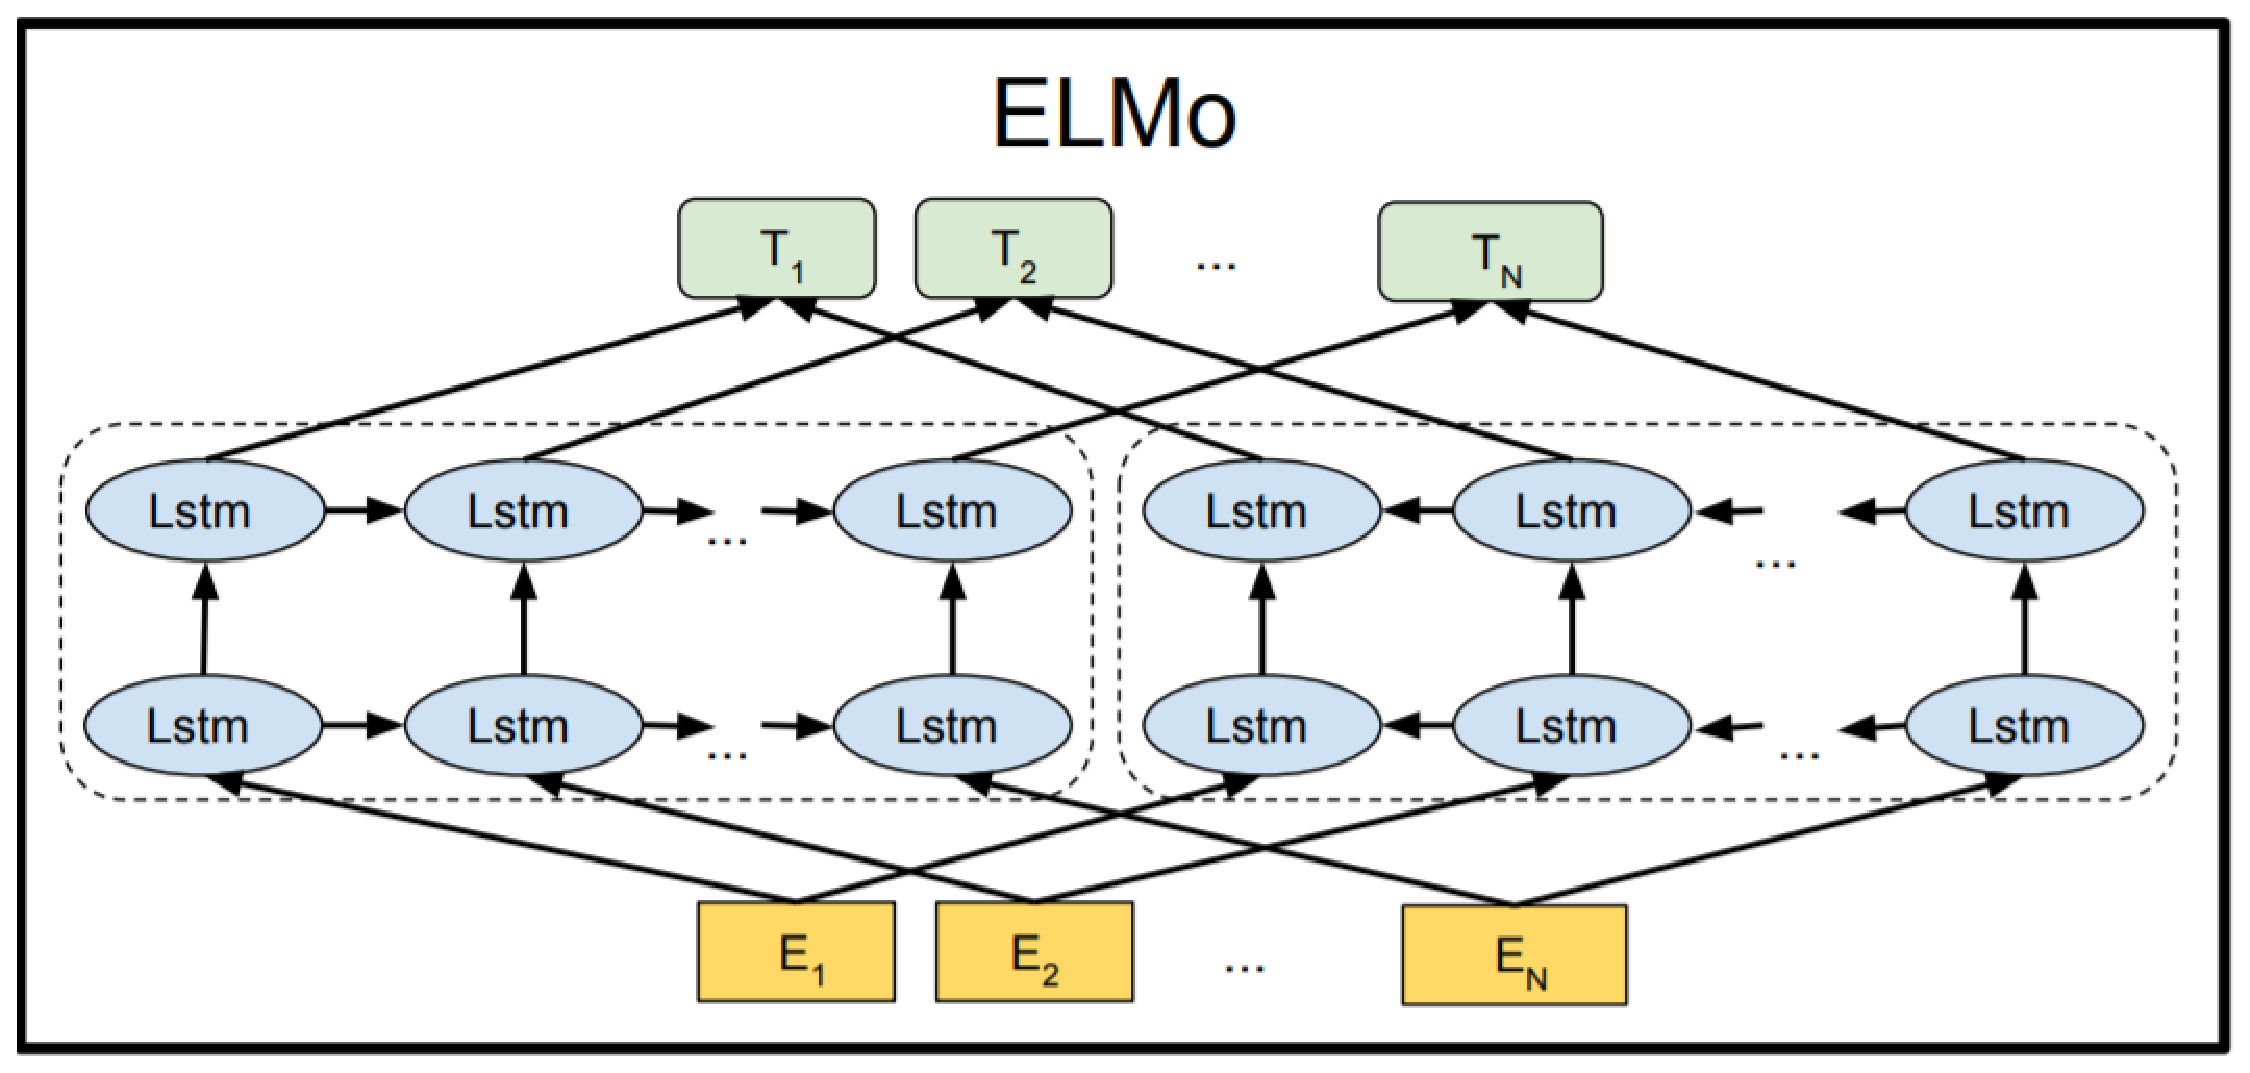
\includegraphics[width=0.95\textwidth]{figures/elmo.eps}

  \footnotesize{\hspace{3.3cm}(Figure from \cite{peters2018deep}).}
  
  \normalsize At first approximation, the context dependent embeddings are all
  the $2n +1 $ intermediate representations produced by the model (one static
  character-based and $2n$ contextual).
  % i.e., the
  % context-independent character-level embeddings and those produced by the $2n$
  % LSTM layers.
\end{slide}

\begin{slide}[toc=]{ELMo cont.}
  Although these vectors together can be considered the "full" ELMo
  representation, for actual downstream NLP tasks ELMo's creators actually
  suggest not to use this very high-dimensional representation, but a lower
  dimensional combination of these vectors. Solutions they suggest are
  \begin{itemize}
  \item simply taking the concatenation of the output of the top LSTM layers (forward
    and backward);
  \item learning a task-specific linear combination of the ELMO representations on
    the supervised task.
  \end{itemize}
\end{slide}

\section{References}

\begin{slide}{References}
  \bibliographystyle{plainnat}
  \nobibliography{nlp_course.bib}
  \begin{footnotesize}

    \bibentry{peters2018deep}.\medskip

  \end{footnotesize}
\end{slide}

% \begin{slide}[toc=]{References cont.}
%   \begin{footnotesize}

%     \bibentry{nivre-nilsson-2005-pseudo}.\medskip

%     \bibentry{nivre2013beyond}.\medskip
    
%   \end{footnotesize}
% \end{slide}

\end{document}

%%% Local Variables:
%%% mode: latex 
%%% TeX-master: t
%%% End:

% LocalWords:  Tokenization Discriminative discriminative
